\documentclass[11pt%
%,draft%
,aspectratio=169%
]{beamer}
%
\usepackage{fontspec}
\defaultfontfeatures{Ligatures=TeX}
%\setsansfont{Liberation Sans}
\usepackage{polyglossia}
\setdefaultlanguage{german}
%
% Alternative template for talks of the Freie Universität Berlin.
% Created by Leonard R. König, <leonard.koenig@fu-berlin.de> following the
% guidelines on www.fu-berlin.de/cd
%
% (c) Leonard König, CC BY 4.0
%
% This template was written against UTF-8 capable LaTeX engines, specifically
% LuaLaTeX.

% Trying to get rather close to the ppt/odp template:
%  http://www.fu-berlin.de/sites/cd/downloads_container/PowerPoint_Praesentation_Anleitung.pdf

%%% font styles
\setbeamerfont{frametitle}{series=\bfseries}
\setbeamerfont{footline}{series=\bfseries}
\setbeamerfont{headline}{series=\bfseries}
\setbeamerfont{alerted text}{series=\bfseries}
%%%

% colordefs
\definecolor{fu_darkblue}{RGB}{0,51,102}
\definecolor{fu_seablue}{RGB}{0,102,204}
\definecolor{fu_lightblue}{RGB}{204,214,224}
\definecolor{fu_green}{RGB}{153,204,0}
\definecolor{fu_lightgrey}{RGB}{128,128,128}
\definecolor{fu_grey}{RGB}{95,95,95}
%
\definecolor{fu_red}{RGB}{204, 0, 0} % red text (used by \alert)
%%% end colordefs

%%% colors
\setbeamercolor*{title}{fg=fu_darkblue}
\setbeamercolor*{subtitle}{fg=fu_seablue}
\setbeamercolor*{frametitle}{fg=fu_darkblue}
\setbeamercolor*{footline}{fg=fu_grey,bg=fu_lightblue}
\setbeamercolor*{headline}{fg=fu_grey}

\setbeamercolor*{normal text}{fg=black}
\setbeamercolor*{alerted text}{fg=fu_red}
\setbeamercolor*{example text}{fg=fu_green}
\setbeamercolor*{structure}{fg=fu_darkblue}

\setbeamercolor*{block title}{fg=white,bg=black!50}
\setbeamercolor*{block title alerted}{fg=white,bg=black!50}
\setbeamercolor*{block title example}{fg=white,bg=black!50}

\setbeamercolor*{block body}{bg=black!10}
\setbeamercolor*{block body alerted}{bg=black!10}
\setbeamercolor*{block body example}{bg=black!10}

\setbeamercolor{bibliography entry author}{fg=fu_darkblue}

\setbeamercolor{item}{fg=fu_darkblue}
\setbeamercolor{navigation symbols}{fg=fu_lightgrey,bg=fu_grey}
%%% end colors

%%% title page
% Display logo (if exists) and right next to it, put our title + subtitle
\defbeamertemplate*{title page}{fu_titlepage}
{%
	\hskip .3\textheight
	\begin{minipage}[.4\textheight]{\textwidth}
		\begin{minipage}[.4\textheight]{0.25\textwidth}
			\inserttitlegraphic
		\end{minipage}%
		\begin{minipage}[.4\textheight]{0.75\textwidth}
			\begin{beamercolorbox}{title}
				\usebeamerfont{title}\inserttitle\par%
			\end{beamercolorbox}
			\vfill
			\ifx\insertsubtitle
				\@empty%
			\else
				\begin{beamercolorbox}{subtitle}
					\usebeamerfont{subtitle}\insertsubtitle\par
				\end{beamercolorbox}
			\fi
		\end{minipage}
	\end{minipage}%
	\hskip .3\textheight
}
%%% end title page

%%% headline
% display title, author and institute on the left;
% logo on the right.
\newcommand{\headlinetext}
{%
	\inserttitle\\[0.3em]%
	\insertauthor, %
	\insertshortinstitute
}
\newlength{\headlinewidth}
\setlength{\headlinewidth}{\paperwidth}
\addtolength{\headlinewidth}{-2\marginparsep}
\setbeamertemplate{headline}
{%
	\begin{beamercolorbox}[wd=\paperwidth]{headline}%
		\vskip5pt
		{\hspace*{\marginparsep}}%
		\parbox{.5\headlinewidth}
		{%
			\usebeamertemplate{title in head/foot}%
			\headlinetext%
		}%
		\begin{minipage}{.5\headlinewidth}%
			\hfill\usebeamertemplate*{logo}
		\end{minipage}%
		{\hspace*{\marginparsep}}%
	\end{beamercolorbox}%
}
%%% end headline

%%% footline
% title + date on the left, frame number on the right
\newcommand{\footlinetext}
{%
	\usebeamerfont{shorttitle}\insertshorttitle, %
	\usebeamerfont{shortdate}\insertshortdate
}
\setbeamertemplate{footline}
{%
	\begin{beamercolorbox}{footline}
		\vskip2pt
		\hspace{\marginparsep}%
		\footlinetext\hfill%
		\insertframenumber%
		\hspace{\marginparsep}
		\vskip2pt
	\end{beamercolorbox}%
}
%%% end footline

% don't use default templates for sidebars
\setbeamertemplate{sidebar right}{}
\setbeamertemplate{sidebar left}{}
\setbeamertemplate{title page}[fu_titlepage]
%
\usepackage{amsmath}
\usepackage{amsfonts}
\usepackage{amssymb}
%
\usepackage{graphicx}

\author{Lea Muth \and Benjamin Tröster}
\title[Code-basierte Kryptografie]{Einführung Code-basierte Kryptografie}
\subtitle{Code-basiertes Kryptosystem -- McEliece}
%\pgfdeclareimage{titlegraphic}{pictures/mceliece.png}
%\titlegraphic{\pgfuseimage{titlegraphic}}
\date{\today}
%\subject{}
%
% FU settings
\institute[FU Berlin]{Freie Universität Berlin}
%\pgfdeclareimage[height=0.9cm]{logo}{../res/dwarf_logo}
%\logo{\pgfuseimage{logo}}
%
\begin{document}

\begin{frame}
\titlepage
\end{frame}

\begin{frame}{Fahrplan}
\tableofcontents[hideothersubsections]
\end{frame}

\section*{Zusammmenfassung}
\begin{frame}{Zusammmenfassung}
	\begin{itemize}
		\item McEliece asymmetrisches Public-Key-Kryptosystem -- 1978 nach Robert McEliece \cite{McEliece1978public}
		\item Grundlegende Idee: Führe absichtliche Fehler in die Chiffre ein 
		\item Verwenden eines allgemeinen fehlerkorrigierende Codes
		\begin{itemize}
		    \item Dekodierung i.A. $\mathcal{NP}$-Hart \cite[S. 479]{Schneier2007Applied}, \cite[S. 353ff]{Stinson2018Cryptography}
		    \item Unterklasse an linearen Codes auch in $P$ lösbar $\rightarrow$ Goppa-Codes
		\end{itemize}
		\item Angreifer ohne Goppa-Code kann nur in $\mathcal{P}$, also polynomiell viel rechnen
		\begin{itemize}
		    \item Die Entschlüsselung eines zufälligen linearen codes ist ein $\mathcal{NP}$-Hartes Problem -> QUELLE!
		    \item Die Generatormatrix eines Goppa-Codes sieht zufällig aus -> QUELLE
		\end{itemize}
	\end{itemize}
\end{frame}

\section{Grundlagen}

\begin{frame}{Fahrplan Grundlagen}
\tableofcontents[currentsection,currentsubsection]
\end{frame}

\begin{frame}{Hamming Gewicht}
	\begin{itemize}
		\item Das Hamming Gewicht eines Vektors $x$ der Länge $n$ ist definiert als:
		       \[ weight_{\Delta}(x):= \sum_{i=1}^n weight_{\Delta}(x_i)  \]
		       \\mit\\ $weight_{\Delta}(x_i) = 1: x_i \neq 0$, \\$weight_{\Delta}(x_i) =0 : x_i = 0$ 
     	\item Beispiel:
					$$
					weight_{\Delta}(\underline{1}00\underline{1})  = 2
					$$
	\end{itemize}
\end{frame}

\subsection{Hamming Distanz}

\begin{frame}{Hamming Distanz}
	\begin{itemize}
		\item Die Hamming Distanz $d$ ist ein Maß für die Unterschiedlichkeit von Zeichenketten und ist eine Metrik auf dem Coderaum.
		\\Es sei $\Sigma$ ein diskretes Alphabet und $c_1=(c_{1_1},\ldots,c_{1_n})$ ,$c_2=(c_{2_1},\ldots,c_{2_n})$ Codeworte mit je $n$ Buchstaben aus $\Sigma^n$, von denen die Teilmenge  $C\subseteq\Sigma^n$ die gültigen Codeworte darstellt. 
		Die Hamming Distanz zwischen $c_1$ und $c_2$ ist definiert als \[\Delta(c_1,c_2):=|\{i \in \{1,\ldots,n\}| c_{1_i}\neq c_{2_i} \}|\]
		\item Beispiel:
					$ 11011001\oplus 10011101 = 0\underline{1}000\underline{1}00 
					\implies \Delta(11011001,10011101) = 2
					$
	\end{itemize}
\end{frame}

\begin{frame}{Hamming Distanz}
	\begin{itemize}
	
		\item Für mehr als zwei Worte versteht man das Minimum aller Abstände zwischen verschiedenen Wörtern innerhalb des Codes als deren Hamming Distanz.
		\[d=\Delta(C):= \min_{\forall i,j \in \{1,\ldots,n\}|i\neq j}\Delta(c_i,c_j)\]
		\item Beispiel:\\
		$ 010\oplus 011 = 00\underline{1}\implies \Delta(010,011) = 1	$\\$ 010\oplus 101 = \underline{1}\underline{1}\underline{1}\implies \Delta(010,101) = 3$\\ $011\oplus 101 = \underline{1}\underline{1}0
		\implies \Delta(011,101) = 2 $\\$d=\min\{1,3,2\}=1$
	\end{itemize}
\end{frame}

\subsection{Linear-Codes}
\begin{frame}{Linear-Codes}
	\begin{itemize}
		\item Ein binärer Blockcode $C\subseteq GF(2^n) \subseteq \Sigma^n$ heißt linearer Code, wenn die Modulo-Summe zweier Codewörter wieder ein Codewort ist, d.h. wenn gilt:
			\[\forall c_1,c_2 \in C \colon c1\oplus c2 \in C \]
			$C$ bildet damit einen Vektorraum und ist Unterraum des Vektorraumes $GF(2^n)$.
		\item Es sei die $k$ die Dimension des Vektorraumes in dem sich der lineare Code $C$ befindet, so nennt man $C$ einen $(n,k)$-Code. Bei gegebener Hamming Distanz $d$ wird dieser auch $(n,k,d)$-Code genannt. 
	\end{itemize}
\end{frame}


\subsection{Goppa-Codes}

\begin{frame}{(binary) Goppa-Codes}
	\begin{itemize}
		\item Ein irreduzibler binärer Goppa-Code ist ein $[n,k,d]$-Code, der durch ein Generatorpolynom $g(x)$ vom Grad $t$ und einer Sequenz $L$ mit $n$ Elementen, über dem endlichen Körper $GF(2^n)$ definiert ist. 
		\item 
	\end{itemize}
\end{frame}

\section{McEliece -- Code-basierte Kryptografie}

\begin{frame}{Fahrplan Code-basierte Kryptografie}
\tableofcontents[currentsection,currentsubsection]
\end{frame}

\begin{frame}{Code-basierte Kryptografie}
	\begin{itemize}
		\item Einleitender Foobar Kram aus: \cite{Stinson2018Cryptography}
	\end{itemize}
	\begin{figure}
	    \centering
	    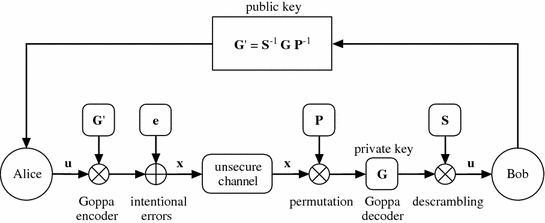
\includegraphics[scale=0.6]{pictures/mceliece.png}
	    \caption{Caption}
	    \label{fig:mceliece_overvie }
	\end{figure}
\end{frame}

\subsection{McEliece-Kryptosystem}

\begin{frame}{Grundlegende Idee McEliece Kryptosystem}
	\begin{itemize}
		\item Transformiere Klartext $m$ (Message) mithilfe einer Generator-Matrix in allgemeinen Goppa-Code
		\item Multiplikation mit randomisierten Matrizen führt zu allgemeinem linearen Code
		\begin{itemize}
		    \item Gist: Reihe von Matrix-Multiplikationen ist Verschlüsselung
		\end{itemize}
		\item Retransformation ohne Matrizen in Goppa-Code ist problemtisch: $\mathcal{NP}$-Hart \cite{Stinson2018Cryptography}
        \item Öffentlicher Schlüssel:
        \begin{itemize}
            \item Beinhaltet Generator-Matrix zur Umwandlung in allg. linearen Code
            \item Zusätzlich: Anzahl der maximal einbaubaren Fehler in der Chiffre $c$
            \item Fehler sind also die Anzahl der Bits, die invertiert werden sollen
        \end{itemize}
	    \item Privater Schlüssel: Umwandlung des allgemeinen, linearen Codes in Goppa-Code
	    \begin{itemize}
	        \item Für performante Retransformation
	        \item Und Fehlerkorrektur
	    \end{itemize}
	\end{itemize}
\end{frame}
 

\subsection{Parameter Definitionen}
\begin{frame}{Parameter Definitionen}
    \begin{itemize}
        \item Systemparameter $m$ gibt die Blockgröße an, für zu verschlüsselnde Nachricht
        \item $C$ sei ein binärer $(n,k)$ Goppa-Code mit $t$ effizient korrigierbaren Fehlern
        \item $t$ gibt die maximale Anz. eff. korrigierbarer Fehler durch Goppa-Code $C$
        \item Daraus ergeben sich:
        \begin{itemize}
            \item Blocklänge Chiffretext: $n = 2^m$
            \item Nachricht Blocklänge $k = n - m \cdot t$
            \item Minimale \emph{Hamming-Distance} $d$ des Codes $C$: $d = 2 \cdot t + 1$
        \end{itemize}
    \end{itemize}   
\end{frame}

\subsection{McEliece Algorithmus}
\begin{frame}{McEliece als Kryptografisches Shema}
    \begin{itemize}
        \item Das \emph{McEliece}-Kryptosystem $\Pi := (Gen, Enc, Dec)$
        \item Wobei:
        \begin{itemize}
            \item $Gen$ Schlüsselerzeugung
            \item $Enc$ Verschlüsselung
            \item $Dec$ Entschlüsselung
        \end{itemize}
        \item Korrekheit: Es muss gelten
        $$
            m = Dec_{priv}(c) = Dec_{priv} (Enc_{pub}(m))
        $$
    \end{itemize}
\end{frame}

\subsection{Schlüsselerzeugung $Gen$}
\begin{frame}{Schlüsselerzeugung $Gen$}
\begin{itemize}
    \item Erzeuge Generator-Matrix $G^{k \times n}$  für Goppa-Code $C$
    \begin{itemize}
        \item Matrix aus der binärer Klartext mit Länge $k$ die Chiffre der Länge $n$ berechnet werden kann
    \end{itemize}
    \item Erzeuge zufällige, binäre, nicht singuläre\footnote{M.a.W. $S$ ist regulär, $\det S \neq 0$; wichtig für Invertierbarkeit} \emph{Scramble-Matrix} $S^{k \times k}$
    \begin{itemize}
        \item $S$ muss in $\mathbb{Z}_2$ invertierbar sein
    \end{itemize}
    \item Permutationsmatrix $P^{n \times n}$
    \begin{itemize}
        \item Binärmatrix, je Zeile genau ein 1 Element enthalten ist
    \end{itemize}
    \item Berechne: $\hat{G}^{k \times n} = S \cdot G \cdot P$
    \item Schlüssel: $K := (G,S,P,\hat{G},t)$\footnote{McEliece fixiert $t=50$, als Maximalwert \cite{McEliece1978public}}
    \begin{itemize}
        \item Öffentlicher Schlüssel: $K_{pub}:= (\hat{G}, t)$
        \item Privater Schlüssel: $K_{priv} := (G,S,P)$
    \end{itemize}
\end{itemize}
\end{frame}

\subsection{Verschlüsselung $Enc$}
\begin{frame}{Verschlüsselung $Enc$}
    \begin{itemize}
        \item Nachricht in Blöcke, sodass $m \in \mathbb{Z}_2^k$
        \item $Enc_{pub}(m,z) = c = m\hat{G} + z$
        \item Sei $z \in \mathbb{Z}_2^n$ ein belieber Vektor der Länge $n$, mit maximaler Gewichtung $t$
        \item Gewichtung $t$: maximale Anzahl Einsen in $z$
        \item Fehlervektor erlaubt es Chiffre an maximal $t$ Stellen zu invertieren
    \end{itemize}
\end{frame}
    
\subsection{Entschlüsselung $Dec$}
\begin{frame}{Entschlüsselung $Dec$}
    \begin{itemize}
        \item Berechne $\hat{c} = cP^{-1}$
        \item Anwenden der $decode(c)$ des Goppa-Codes auf $\hat{c}$, sodass $\hat{m}$ gefunden werden kann
        \item Hamming-Distanz: $d_H(\hat{m}G, \hat{c}) \leq t$
        \item Eigentliche Entschlüsselung: $m = \hat{m}S^{-1}$
        \item Kompakt: $dec_{priv}(c) = decode(cP^{-1}) \cdot S^{-1}$
    \end{itemize}    
\end{frame}

\subsection{Beispiel McElicece-Kryptosystem}
\begin{frame}{Beispiel McElicece-Kryptosystem}
    \begin{itemize}
        \item Kryptosystem $(n,k,d)$ mit Systmeparameter: $n=7, k=4, d=3$
        \begin{itemize}
            \item 4 Bit Klartext auf $7$ Bit Chiffretext
            \item Hamming-Distanz $d=3$
            \item Somit lassen sich $t = \frac{d-1}{2} = 1$ Bitfehler korrigieren
        \end{itemize}
    \end{itemize}
\end{frame}

\begin{frame}{Beispiel McElicece-Kryptosystem, cont'}
    \begin{itemize}
        \item Schlüsselerzeugung $Gen$: Generator-Matrix erzeugt Hamming-Code statt Goppa-Code
        \item $G=\begin{pmatrix} 1 & 0 & 0 & 0 & 1 & 1 & 0 \\ 0 & 1 & 0 & 0 & 1 & 0 & 1 \\ 0 & 0 & 1 & 0 & 0 & 1 & 1 \\ 0 & 0 & 0 & 1 & 1 & 1 & 1 
        \end{pmatrix}$\\
        Da $d=3$ unterscheidet sich jede Zeile in mindestens drei Werten
        \item Zufällige Matrizen $S$ und $P$
        $S=\begin{pmatrix} 1 & 1 & 0 & 1 \\ 1 & 0 & 0 & 1 \\ 0 & 1 & 1 & 1 \\ 1 & 1 & 0 & 0 \end{pmatrix} \qquad
        P=\begin{pmatrix} 0 & 1 & 0 & 0 & 0 & 0 & 0 \\ 0 & 0 & 0 & 1 & 0 & 0 & 0 \\ 0 & 0 & 0 & 0 & 0 & 0 & 1 \\ 1 & 0 & 0 & 0 & 0 & 0 & 0 \\ 0 & 0 & 1 & 0 & 0 & 0 & 0 \\ 0 & 0 & 0 & 0 & 0 & 1 & 0 \\ 0 & 0 & 0 & 0 & 1 & 0 & 0 \end{pmatrix}$
    \end{itemize}
\end{frame}

\begin{frame}{Beispiel McElicece-Kryptosystem, cont'}
Berechnung des öffentlichen Schlüssels $\hat{G} = S \cdot G \cdot P$:
$$
    \hat{G}=\begin{pmatrix} 1 & 1 & 0 & 1 \\ 1 & 0 & 0 & 1 \\ 0 & 1 & 1 & 1 \\ 1 & 1 & 0 & 0 \end{pmatrix} \cdot \begin{pmatrix} 1 & 0 & 0 & 0 & 1 & 1 & 0 \\ 0 & 1 & 0 & 0 & 1 & 0 & 1 \\ 0 & 0 & 1 & 0 & 0 & 1 & 1 \\ 0 & 0 & 0 & 1 & 1 & 1 & 1 \end{pmatrix} \cdot \begin{pmatrix} 0 & 1 & 0 & 0 & 0 & 0 & 0 \\ 0 & 0 & 0 & 1 & 0 & 0 & 0 \\ 0 & 0 & 0 & 0 & 0 & 0 & 1 \\ 1 & 0 & 0 & 0 & 0 & 0 & 0 \\ 0 & 0 & 1 & 0 & 0 & 0 & 0 \\ 0 & 0 & 0 & 0 & 0 & 1 & 0 \\ 0 & 0 & 0 & 0 & 1 & 0 & 0 \end{pmatrix}=
$$
\end{frame}

\begin{frame}{Beispiel McElicece-Kryptosystem, cont'}
Berechnung des öffentlichen Schlüssels $\hat{G} = S \cdot G \cdot P$:
$$
    =\begin{pmatrix} 1 & 1 & 0 & 1 & 1 & 0 & 0 \\ 1 & 0 & 0 & 1 & 0 & 0 & 1 \\ 0 & 1 & 1 & 1 & 0 & 0 & 1 \\ 1 & 1 & 0 & 0 & 0 & 1 & 1 \end{pmatrix} \cdot \begin{pmatrix} 0 & 1 & 0 & 0 & 0 & 0 & 0 \\ 0 & 0 & 0 & 1 & 0 & 0 & 0 \\ 0 & 0 & 0 & 0 & 0 & 0 & 1 \\ 1 & 0 & 0 & 0 & 0 & 0 & 0 \\ 0 & 0 & 1 & 0 & 0 & 0 & 0 \\ 0 & 0 & 0 & 0 & 0 & 1 & 0 \\ 0 & 0 & 0 & 0 & 1 & 0 & 0 \end{pmatrix}= \begin{pmatrix} 1 & 1 & 1 & 1 & 0 & 0 & 0 \\ 1 & 1 & 0 & 0 & 1 & 0 & 0 \\ 1 & 0 & 0 & 1 & 1 & 0 & 1 \\ 0 & 1 & 0 & 1 & 1 & 1 & 0 \end{pmatrix}
$$
\end{frame}

\begin{frame}{Beispiel McElicece-Kryptosystem, cont'}
Der öffentlichen Schlüssels $K_{pub} = (\hat{G},t)$:
$$
    K_{pub} = (\hat{G},t) =\left(\begin{pmatrix} 1 & 1 & 1 & 1 & 0 & 0 & 0 \\ 1 & 1 & 0 & 0 & 1 & 0 & 0 \\ 1 & 0 & 0 & 1 & 1 & 0 & 1 \\ 0 & 1 & 0 & 1 & 1 & 1 & 0 \end{pmatrix},1\right)
$$
\end{frame}

\begin{frame}{Beispiel McElicece-Kryptosystem, cont'}
Nachricht $m = \begin{pmatrix} 1 1 0 1 \end{pmatrix}$, Fehlervektor $z$ mit maximalem Gewicht $t = 1$ und Länge $n = 7$: \\
Wähle $z =  \begin{pmatrix} 0 0 0 0 1 0 0 \end{pmatrix}$ 
$$
    Enc_{pub}(m,z) = c = m\hat{G} + z
$$
\begin{align*}
    m &= \begin{pmatrix} 1 & 1 & 0 & 1 \end{pmatrix} \cdot \begin{pmatrix} 1 & 1 & 1 & 1 & 0 & 0 & 0 \\ 1 & 1 & 0 & 0 & 1 & 0 & 0 \\ 1 & 0 & 0 & 1 & 1 & 0 & 1 \\ 0 & 1 & 0 & 1 & 1 & 1 & 0 \end{pmatrix} + \begin{pmatrix} 0 & 0 & 0 & 0 & 1 & 0 & 0 \end{pmatrix}\\
    &= \begin{pmatrix} 0 & 1 & 1 & 0 & 0 & 1 & 0 \end{pmatrix} + \begin{pmatrix} 0 & 0 & 0 & 0 & 1 & 0 & 0 \end{pmatrix}\\
    &= \begin{pmatrix} 0 & 1 & 1 & 0 & 1 & 1 & 0 \end{pmatrix}=c    
\end{align*}
\end{frame}

\begin{frame}{Beispiel McElicece-Kryptosystem, cont'}
Entschlüsselung der Chiffre:\\
Invertierung der Permuation $\hat{c} = cP^{-1}$
\begin{align*}
       c &= \begin{pmatrix} 0 & 1 & 1 & 0 & 1 & 1 & 0 \end{pmatrix} \cdot \begin{pmatrix} 0 & 0 & 0 & 1 & 0 & 0 & 0 \\ 1 & 0 & 0 & 0 & 0 & 0 & 0 \\ 0 & 0 & 0 & 0 & 1 & 0 & 0 \\ 0 & 1 & 0 & 0 & 0 & 0 & 0 \\ 0 & 0 & 0 & 0 & 0 & 0 & 1 \\ 0 & 0 & 0 & 0 & 0 & 1 & 0 \\ 0 & 0 & 1 & 0 & 0 & 0 & 0 \end{pmatrix}\\
       &= \begin{pmatrix} 1 & 0 & 0 & 0 & 1 & 1 & 1 \end{pmatrix}
\end{align*}
\end{frame}

\begin{frame}{Beispiel McElicece-Kryptosystem, cont'}
\begin{itemize}
    \item Dekodierung des Hamming-Codes:
    \item Berehcne Hamming-Distanz $d$ der Generator-Matrix $G$: $\begin{pmatrix} 1 & 3 & 3 & 2 \end{pmatrix}$
    \item Somit ist $\hat{m} = \begin{pmatrix} 1 & 0 & 0 & 0\end{pmatrix}$
    \item Berechne Klartext $m$
\end{itemize}

\begin{align*}
        m &= \hat{m}S^{-1}=\\
        &= \begin{pmatrix} 1 & 0 & 0 & 0 \end{pmatrix} \cdot \begin{pmatrix} 1 & 1 & 0 & 1 \\ 1 & 1 & 0 & 0 \\ 0 & 1 & 1 & 1 \\ 1 & 0 & 0 & 1 \end{pmatrix}\\
        &= \begin{pmatrix} 1 & 1 & 0 & 1 \end{pmatrix}
\end{align*}
\end{frame}

\subsection{Vor- \& Nachteile}
\begin{frame}{Vor- \& Nachteile}
    \begin{itemize}
        \item The good news: Es gab keine erfolgreichen Angriffe gegen das McEliece-Verfahren
        \item Verhfahren gilt als  \emph{IND-CCA2} \cite{dottling2012cca2} sicher, somit ist es auch \emph{IND-CPA} sicher \cite{nojima2008semantic}
        \item Angriffe McEliece mit originalen Parametern von 1978 in 1400 Tagen (Einzelne Machine) oder in 7 Tagen mithilfe von 200 CPUs \cite{baldi2016enhanced}, \cite{canteaut1998cryptanalysis}
        \item Jedoch:
        \begin{itemize}
            \item Bruce Schneier: McEliece-Kryptosystem etwa 2 bis 3 mal langsamer als RSA \cite[S. 479ff]{Schneier2007Applied}
            \item Extrem große öffentliche Schlüssel: $\hat{G}$ ist Matrix $k \times n$
            \item Bei Parameter $(1024,524,101)$ ist $k \cdot n = 1024 \cdot 524 = 536576$ Bit also etwa 67$kBytes$
            \item Chiffretext ist fast doppelt so groß wie Klartext, aus $524 Bit$ klartext werden zu $1024$ Bit Chiffre 
        \end{itemize}
     \end{itemize}
\end{frame}

\section{Quellen}
\appendix
\begin{frame}[allowframebreaks]
  \frametitle<presentation>{Sources}
\bibliographystyle{alpha}
\bibliography{sources}
\end{frame}
\end{document}